\section{Resultat}
\label{sec:joel_a-results}
I denna del ska alla produktens miljökonsekvenser eliciteras. 

\subsection{Nivå ett effekter}
Nivå ett effekter i Greensoft modellen är de effekter som direkt följer av utvecklingen eller användningen av produkten. Dessa är de enda effekterna som tas upp i detta kapitel då det är de enda effekterna som kan ha uppkommit. Nivå två och tre effekter kan först uppkomma efter användning av produkten, något som vid skrivandets stund inte skett. Den första fasen i Greensoft modellen är utvecklingsfasen och i den kan följande nivå ett effekter hittas:
\begin{itemize}
	\item Strömanvändning för utvecklarnas datorer
	\item Övrig strömanvändning av utvecklarna
	\item Transport till arbetsplats
	\item Bredbandet och molntjänster utvecklarna använde sig av under utvecklingen
\end{itemize}

Transporten till arbetsplatsen skedde uteslutande med cyckel och gång så denna punkt bidrog inte till någon mätbar miljöpåverkan.

\subsubsection{Strömanvändning}
Projektet att skapa produkten ingick i en större universitetskurs som tog 3200 arbetstimmar för hela gruppen, uppskattningsvis kan åtminstone hälften av denna tit sägas ha lagts på produkten. Gruppen bestod av åtta personer som framförallt arbetade med produkten på sina laptops. All utvecklingstid gjordes dock inte vid en dator, visa moment såsom skapandet av arkitekturen och gruppmöten så användes ingen dator. Dessutom så skedde delar av utveckling med flera gruppmedlemmar vid samma dator. För att få in detta i uppskattningen kan vi säga att 90\% av utvecklingstiden skedde med en laptop. Så totalt blir strömanvändningen 1600 * 8 * 0.9 * x, där x står för den genomsnittliga strömanvändningen för en laptop. Eftersom en laptops strömanvändning beror på så många faktorer är det svårt att få en korrekt uppskattning av hur mycket ström som används. En ungefär värde på x kan fås genom observationen att en av medlemmarnas laptop kunde användas i ungefär fyra timmar innan den behövde laddas. Denna laptop är av modell ''Lenovo ideapad Y700'' och har enligt tillverkaren \cite{lenovo} ett batteri med 60 watt timmar. En urladdning på av detta på fyra timmar ger oss en timmes användning av 15 watt, vilket x kan approximeras till. Då får vi följande approximering för strömanvändning av datorerna gruppen använde sig av under utecklingsprocessen: $$1600 * 8 * 0.9 * 15 = 172.8kW$$

Utvecklarnas övriga strömanvändninge kommer framförallt ifrån strömanvändning i rummet där utvecklingen sker, saker såsom belysning, ventilation, och uppvärmning. Uppvärmningen av rummet kan ignoreras i detta fall då alla rum gruppen arbetade i skulle varit uppvärmda oavsett ifall de befann sig där eller inte. I stort sett all utveckling skedde i arbetsrum på Linköpings Universitet som är uppvärmda oavsett ifall de används och kontoret på Cybercom som också skulle vara uppvärmt oavsett gruppens närvaro. I energimyndighetens rapport ifrån 2007\cite{emynd} så använder det genomsnittliga svenska kontoret $23.0kWh/m^2$ för belysning och $2.6kWh/m^2$ för ventilation. En approximering av storleken på rummen gruppen arbetade i är 15 kvadratmeter, vilket ger oss en ungefärlig strömanvändning på: $$1600 * 25.6 * 15 = 614.4kW$$

\subsubsection{Molntjänster}
Under utvecklingsprocessen använde sig teamet av flertal olika molntjänster såsom Google drive, Github och Googles sökmotor. Teamet uppskattas göra en Google-sökning var tionde utvecklingsminut eller sex sökningar per timme, vilket ger oss $1600 * 6 = 9600$ sökningar. I tabellen \ref{tab:drive_results_table} så redovisas teamets Google drive historik och i tabell \ref{tab:github_results_table} Github historiken. Enligt metoden så uppskattas dessa operationer släppa ut trippelt så mycket koldioxid som en Googlesökning som ligger på 0.2 gram per sökning\cite{google-blog}. Då får vi ett uppskattat koldioxid utsläpp på: $$9600 * 0.2 + 0.6 * (136 + 577) = 2347.8\text{ gram \ce{CO2}}$$



\begin{table}
	\centering
	\begin{tabular}{| l | l |}
		\cline{1-2}
		\multicolumn{1}{| c |}{\textbf{Operation}} & \textbf{Antal}  \\ \hline
		Redigera & 262 \\ \hline
		Kopiera & 43 \\ \hline
		Kommentera & 4 \\ \hline
		Byta namn & 40 \\ \hline
		Ladda upp & 95 \\ \hline
		Skapa & 92 \\ \hline
		Flytta & 39 \\ \hline
		Ta bort & 2 \\ \hline
		\textbf{Totalt} & \textbf{577}\\ \hline
	\end{tabular}
	\caption{Antal operationer teamet gjort på Google drive}
	\label{tab:drive_results_table}
\end{table}



\begin{table}
	\centering
	\begin{tabular}{| l | l |}
		\cline{1-2}
		\multicolumn{1}{| c |}{\textbf{Gitrepo}} & \textbf{Antal push operationer}\\ \hline
		UI & 31 \\ \hline
		Kontroller & 26 \\ \hline
		Services & 12 \\ \hline
		Dokument & 67 \\ \hline
		Server & 0 \\ \hline
		\textbf{Totalt} & \textbf{136} \\ \hline
	\end{tabular}
	\caption{Antal git push operationer som gruppen gjort mot huvudgrenen på Githubs hemsida}
	\label{tab:github_results_table}
\end{table}



\begin{figure*}[h]
	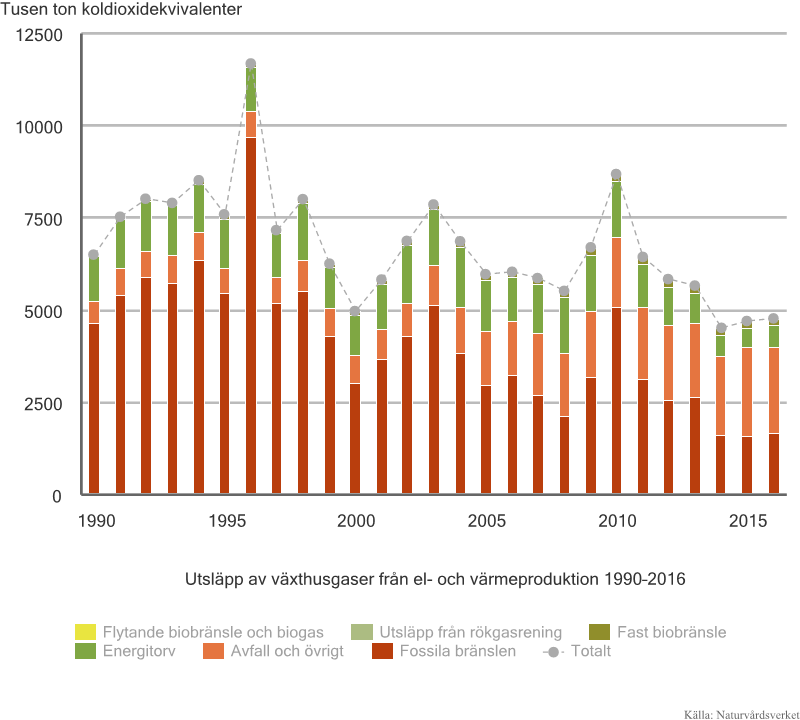
\includegraphics[scale=0.7]{naturvard-co2}
	\caption{Statistik ifrån naturvårdsverket}
	\label{natuvard-co2}
\end{figure*}


\subsection{Miljöpåverkan av utvecklingsprocessen}
Enligt \ref{natuvard-co2} så skapade Sveriges el och värmeproduktion ett \ce{CO2} utsläpp på $4781*10^9$ gram år 2016. Kombinerat med att Sveriges energi produktion detta år var 152 TWh enligt Energimyndighetens pressmeddelande\cite{elprod2016}, så får vi att varje kWh i genomsnitt skapade ett utsläpp på: $4781*10^9 / (152 * 10^{12}) \approx 31.45 * 10^{-3}$ gram \ce{CO2} per kWh. Ifrån tidigare approximerades gruppens kWh till $172.8 + 614.4 = 787.2$ vilket ger oss ett \ce{CO2} utsläpp på: $$31.45 * 10^{-3} * 787.2 \approx 24.8 \text{ gram \ce{CO2}}$$
